% Shared style for all Git & GitHub lectures (same look as the N-body course)
\documentclass[11pt,a4paper]{article}
\usepackage[margin=2.3cm]{geometry}
\usepackage[T1]{fontenc}
\usepackage{lmodern}
\usepackage{upquote}   % straight quotes in monospaced text, so commands can be copied
\usepackage{microtype}
% keep '--' as two real hyphens in monospace text (commands like --version)
\DisableLigatures[-,<,>]{family=tt*}
\usepackage{booktabs,enumitem,graphicx,xcolor}
\usepackage{array}
\usepackage{needspace}
\usepackage{longtable}
\usepackage{float}
\usepackage{tikz}
\usetikzlibrary{arrows.meta,calc,positioning,decorations.pathreplacing,shapes.geometric,fit,backgrounds}
\usepackage[most]{tcolorbox}
\usepackage{listings}
\usepackage{fancyhdr}
\usepackage[colorlinks=true,linkcolor=blue!50!black,urlcolor=blue!50!black,citecolor=blue!50!black]{hyperref}

\setlength{\parindent}{0pt}
\setlength{\parskip}{0.6em}
\setlength{\abovecaptionskip}{4pt}
\usepackage[font=small,labelfont=bf]{caption}
\setlist{itemsep=0.2em,topsep=0.3em}

% ---------- colours ----------
\definecolor{cbg}{HTML}{F6F8FA}
\definecolor{ckw}{HTML}{0B5CAD}
\definecolor{ccm}{HTML}{6A737D}
\definecolor{cst}{HTML}{B5451B}
\definecolor{cpart}{HTML}{1F6FB2}
\definecolor{cheavy}{HTML}{C0392B}
\definecolor{cgreen}{HTML}{2E8B57}

% ---------- terminal listings ----------
% In a terminal session, lines starting with "$" are what YOU type.
% Everything else is what Git prints back.
\lstdefinestyle{term}{
  basicstyle=\ttfamily\small, backgroundcolor=\color{cbg},
  frame=single, rulecolor=\color{black!15}, showstringspaces=false,
  breaklines=true, columns=fullflexible, keepspaces=true,
  aboveskip=0.6em, belowskip=0.6em, xleftmargin=4pt, xrightmargin=4pt,
  literate={\$\ }{{\textcolor{cgreen}{\$\ }}}2,
  upquote=true
}
\lstset{style=term}
\newcommand{\code}[1]{\texttt{\small #1}}

% ---------- boxes ----------
\newtcolorbox{history}{colback=yellow!8,colframe=orange!60!black,
  title={History},fonttitle=\bfseries\small,left=4pt,right=4pt,top=2pt,bottom=2pt}
\newtcolorbox{quickfact}{colback=purple!4,colframe=purple!55!black,
  title={Quick fact},fonttitle=\bfseries\small,left=4pt,right=4pt,top=2pt,bottom=2pt}
\newtcolorbox{keyidea}{colback=blue!4,colframe=blue!50!black,
  title={Key idea},fonttitle=\bfseries\small,left=4pt,right=4pt,top=2pt,bottom=2pt}
\newtcolorbox{pitfall}{colback=red!4,colframe=red!55!black,
  title={Pitfall},fonttitle=\bfseries\small,left=4pt,right=4pt,top=2pt,bottom=2pt}
\newtcolorbox{tryit}{colback=teal!5,colframe=teal!55!black,
  title={Try it},fonttitle=\bfseries\small,left=4pt,right=4pt,top=2pt,bottom=2pt,breakable}
\newtcolorbox{homework}[1]{colback=green!4,colframe=green!40!black,
  title={Homework #1},fonttitle=\bfseries\small,left=4pt,right=4pt,top=2pt,bottom=2pt,
  breakable}
\newtcolorbox{goals}{colback=gray!6,colframe=gray!60!black,
  title={Learning goals},fonttitle=\bfseries\small,left=4pt,right=4pt,top=2pt,bottom=2pt}

% Solutions always start on a fresh page, behind a clear warning.
\newcommand{\solutionspage}{%
  \clearpage
  \begin{tcolorbox}[colback=red!6,colframe=red!60!black,halign=center]
    {\Large\bfseries Solutions}\\[0.3em]
    {\small Stop here if you have not tried the homework yet.\\
    Attempt every task first, run the checker, and only then read on.}
  \end{tcolorbox}
}

% ---------- Git diagram styles (TikZ) ----------
\tikzset{
  commit/.style={circle,draw=black!70,fill=blue!10,minimum size=7mm,inner sep=0pt,font=\scriptsize\ttfamily},
  newcommit/.style={commit,fill=orange!25,dashed},
  tag/.style={draw,rounded corners=2pt,font=\scriptsize\ttfamily,inner sep=2pt},
  branchtag/.style={tag,fill=green!15,draw=green!40!black},
  headtag/.style={tag,fill=yellow!30,draw=orange!70!black},
  remotetag/.style={tag,fill=purple!10,draw=purple!60!black},
  area/.style={draw,rounded corners,minimum height=11mm,minimum width=33mm,align=center,font=\small},
  cmdarrow/.style={->,thick,>=Stealth},
  link/.style={->,thick,>=Stealth,black!70},
}

% ---------- header ----------
\pagestyle{fancy}
\fancyhf{}
\renewcommand{\headrulewidth}{0.3pt}
\fancyfoot[C]{\thepage}
\newcommand{\lecturetitle}[3]{%
  \fancyhead[L]{\small\textit{Git \& GitHub from Zero}}
  \fancyhead[R]{\small Lecture #1}
  \begin{center}
    {\Large\bfseries Lecture #1}\\[0.4em]
    {\LARGE\bfseries #2}\\[0.4em]
    {\small #3}
  \end{center}
  \vspace{0.5em}
}

\tikzset{
  cbx/.style={draw,rounded corners,fill=blue!6,minimum width=2.1cm,minimum height=9mm,align=center,font=\scriptsize\ttfamily,inner sep=2pt}}
\begin{document}
\lecturetitle{5}{Merging Branches and Resolving Conflicts}{Fast-forward merges, merge commits, conflict markers, and \texttt{git merge --abort}}

\begin{goals}
\begin{itemize}
  \item Merge one branch into another and say which kind of merge Git performed.
  \item Explain why a merge commit has two parents, and how Git combines two lines of work.
  \item Read the conflict markers in a file and resolve a conflict step by step.
  \item Cancel a merge safely with \code{git merge --abort}.
  \item Delete branches once they are merged.
\end{itemize}
\end{goals}

\section{What merging means}

In Lecture 4 you created branches and let the history fork. \textbf{Merging} is the other half of the story: bringing the commits of one branch into another, so that the finished work ends up on \code{main}.

The command is \code{git merge}, and its direction matters:

\begin{keyidea}
You first \emph{switch to the branch that should receive the work}, then run \code{git merge <other-branch>}. The current branch changes; the other branch is left untouched. \code{git merge waffles} while on \code{main} means ``bring \code{waffles} into \code{main}''.
\end{keyidea}

Before every merge, get into the habit of two checks: \code{git status} (the working directory should be clean, with everything committed) and \code{git branch --show-current} (you must be on the receiving branch).

For this lecture we use a practice repository with the same starting point on every computer. From the course folder run:

\begin{lstlisting}
$ bash codeHints/L05/setup_demo5.sh
$ cd practice/demo5
$ git log --oneline --graph --all --decorate
* fbed2d3 (vanilla) Pancakes with vanilla
| * 0725dd2 (syrup) Pancakes with syrup
|/
| * 633affa (shopping) Add shopping list
|/
| * df478ec (crepes) Add crepe recipe
|/
* 7ad9635 (HEAD -> main) Add pancake recipe
* 3f587ea Add README
\end{lstlisting}

\code{main} has two commits, and four branches start from its tip. We will merge them one after another, and each one teaches a different case. (To restart at any time: leave the folder with \code{cd ../..}, run \code{setup\_demo5.sh --reset}, then \code{cd practice/demo5}.)

\section{Case 1: the fast-forward merge}

The branch \code{crepes} added one commit on top of \code{main}'s latest commit, and \code{main} has not moved since. Nothing needs combining: Git only has to slide the \code{main} label forward.

\begin{lstlisting}
$ git merge crepes
Updating 7ad9635..df478ec
Fast-forward
 crepes.txt | 1 +
 1 file changed, 1 insertion(+)
 create mode 100644 crepes.txt
\end{lstlisting}

\begin{figure}[H]
\centering
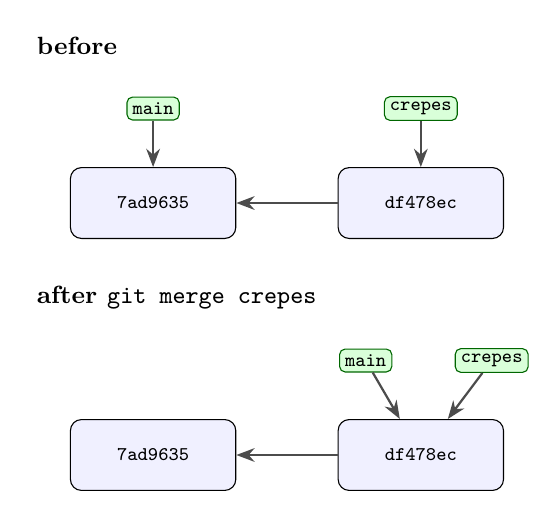
\begin{tikzpicture}
  \node[font=\small\bfseries,anchor=west] at (-1.6,2.0) {before};
  \node[cbx] (a1) at (0,0)   {7ad9635};
  \node[cbx] (b1) at (3.4,0) {df478ec};
  \draw[link] (b1)--(a1);
  \node[branchtag] (m1) at (0,1.2) {main}; \draw[link] (m1)--(a1);
  \node[branchtag] (c1) at (3.4,1.2) {crepes}; \draw[link] (c1)--(b1);
  \node[font=\small\bfseries,anchor=west] at (-1.6,-1.2) {after \code{git merge crepes}};
  \node[cbx] (a2) at (0,-3.2)   {7ad9635};
  \node[cbx] (b2) at (3.4,-3.2) {df478ec};
  \draw[link] (b2)--(a2);
  \node[branchtag] (m2) at (2.7,-2.0) {main}; \draw[link] (m2)--(b2);
  \node[branchtag] (c2) at (4.3,-2.0) {crepes}; \draw[link] (c2)--(b2);
\end{tikzpicture}
\caption{A fast-forward merge. No new commit is created: the \code{main} label just moves forward to the commit \code{crepes} already points at. The history stays a straight line.}
\label{fig:ff}
\end{figure}

\begin{quickfact}
A fast-forward is possible only when the receiving branch has \emph{no commits of its own} beyond the shared starting point. If you ever want a visible merge commit even then, use \code{git merge --no-ff}.
\end{quickfact}

\section{Case 2: the merge commit}

Next, \code{shopping}. It also started from the old \code{Add pancake recipe} commit, but \code{main} has moved on (it now has the crepe commit). The two lines of work have diverged, so Git cannot just slide a label. It must \emph{combine} them:

\begin{lstlisting}
$ git merge --no-edit shopping
Merge made by the 'ort' strategy.
 shopping.txt | 2 ++
 1 file changed, 2 insertions(+)
 create mode 100644 shopping.txt
\end{lstlisting}

(The word \code{ort} is just the name of Git's merging method; older versions print \code{recursive}. Ignore it. Without \code{--no-edit}, Git opens a text editor so that you can confirm the merge message: save and close it, which in \code{vim} means pressing \code{Esc}, typing \code{:wq} and Enter. We skip the editor with \code{--no-edit}.)

Git made a \textbf{merge commit}, a special commit with \emph{two parents} (two commits directly before it): one from each line of work.

\begin{figure}[H]
\centering
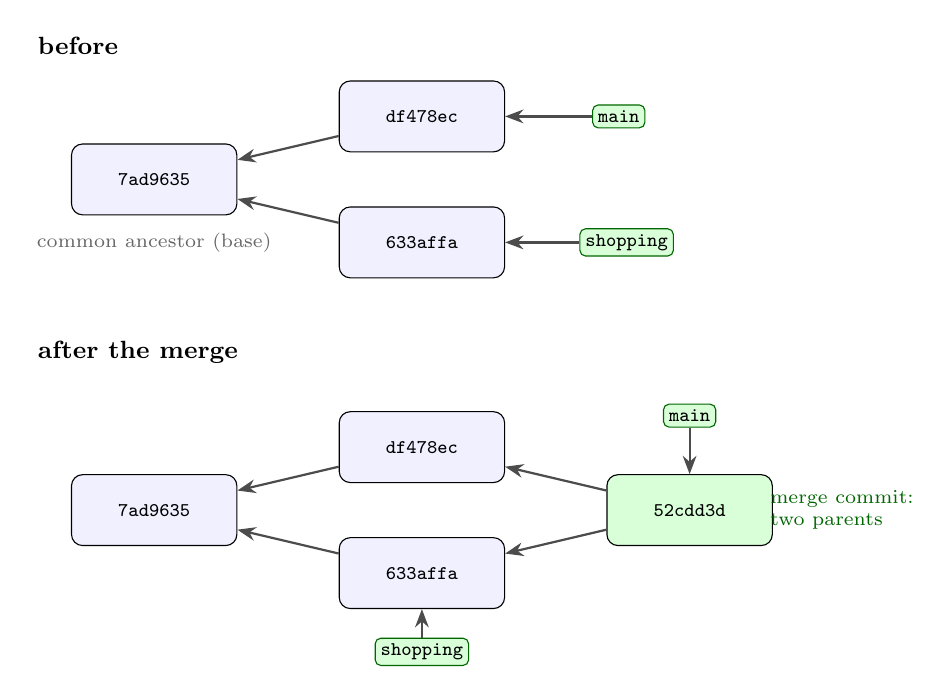
\begin{tikzpicture}
  \node[font=\small\bfseries,anchor=west] at (-1.6,1.7) {before};
  \node[cbx] (p1) at (0,0) {7ad9635};
  \node[cbx] (m1) at (3.4,0.8) {df478ec};
  \node[cbx] (s1) at (3.4,-0.8) {633affa};
  \draw[link] (m1)--(p1); \draw[link] (s1)--(p1);
  \node[branchtag] (mt1) at (5.9,0.8) {main}; \draw[link] (mt1)--(m1);
  \node[branchtag] (st1) at (6.0,-0.8) {shopping}; \draw[link] (st1)--(s1);
  \node[font=\scriptsize,text=black!60,anchor=north] at (0,-0.55) {common ancestor (base)};
  \node[font=\small\bfseries,anchor=west] at (-1.6,-2.2) {after the merge};
  \node[cbx] (p2) at (0,-4.2) {7ad9635};
  \node[cbx] (m2) at (3.4,-3.4) {df478ec};
  \node[cbx] (s2) at (3.4,-5.0) {633affa};
  \node[cbx,fill=green!15] (x2) at (6.8,-4.2) {52cdd3d};
  \draw[link] (m2)--(p2); \draw[link] (s2)--(p2);
  \draw[link] (x2)--(m2); \draw[link] (x2)--(s2);
  \node[branchtag] (mt2) at (6.8,-3.0) {main}; \draw[link] (mt2)--(x2);
  \node[branchtag] (st2) at (3.4,-6.0) {shopping}; \draw[link] (st2)--(s2);
  \node[font=\scriptsize,text=green!40!black,anchor=west,align=left] at (7.7,-4.2) {merge commit:\\two parents};
\end{tikzpicture}
\caption{A three-way merge. Git finds the common ancestor of the two branches and creates a merge commit whose two parents are the two tips. \code{main} moves onto it; \code{shopping} stays where it was.}
\label{fig:threeway}
\end{figure}

The name \emph{three-way} comes from the three versions Git looks at: the common ancestor (the \textbf{base}) and the two branch tips. It compares each tip with the base to see what each side changed, then combines the changes. The rules are simple:

\begin{center}
\small
\begin{tabular}{@{}l l@{}}
\toprule
What happened since the base & Result \\
\midrule
only one side changed a part of a file & Git takes that side's change \\
both sides changed \emph{different, non-adjacent} parts of a file & Git applies both changes \\
both sides changed the \emph{same part} differently & \textbf{conflict}: Git asks you \\
\bottomrule
\end{tabular}
\end{center}

Look at the history, and at the two parents of the merge commit:

\begin{lstlisting}
$ git log --oneline --graph --decorate -4
*   52cdd3d (HEAD -> main) Merge branch 'shopping'
|\
| * 633affa (shopping) Add shopping list
* | df478ec (crepes) Add crepe recipe
|/
* 7ad9635 Add pancake recipe
$ git log -1 --format="%h parents: %p"
52cdd3d parents: df478ec 633affa
$ git log --merges --oneline
52cdd3d Merge branch 'shopping'
\end{lstlisting}

(The ID of any merge commit depends on the time you run the merge, so yours will differ from \code{52cdd3d}. The IDs of the branch commits are fixed.) The command \code{git log --merges} lists only merge commits.

\Needspace{9\baselineskip}
\textbf{One more merge before the conflict.} Merge \code{syrup} now (the next case needs it). It changes line~1 of \code{recipes.txt}, and nothing on \code{main} has touched that file, so Git applies the change on its own and makes a second merge commit:

\begin{lstlisting}
$ git merge --no-edit syrup
Merge made by the 'ort' strategy.
 recipes.txt | 2 +-
 1 file changed, 1 insertion(+), 1 deletion(-)
$ cat recipes.txt
Pancakes: flour, milk, eggs, syrup
\end{lstlisting}

\Needspace{14\baselineskip}
\section{Case 3: the conflict}

Now the branch we have been waiting for. \code{main} (through \code{syrup}) and \code{vanilla} both changed the \emph{same line} of \code{recipes.txt}. Git cannot know which version you want:

\begin{lstlisting}
$ git merge vanilla
Auto-merging recipes.txt
CONFLICT (content): Merge conflict in recipes.txt
Automatic merge failed; fix conflicts and then commit the result.
\end{lstlisting}

\begin{keyidea}
A conflict is not an error and nothing is broken. It is Git saying: ``Both sides edited this spot. A human has to decide.'' The merge is paused halfway, waiting for you. Your earlier commits are completely safe.
\end{keyidea}

\subsection{Step 1: see what is going on}

\begin{lstlisting}
$ git status
On branch main
You have unmerged paths.
  (fix conflicts and run "git commit")
  (use "git merge --abort" to abort the merge)

Unmerged paths:
  (use "git add <file>..." to mark resolution)
	both modified:   recipes.txt

no changes added to commit (use "git add" and/or "git commit -a")
$ git status --short
UU recipes.txt
\end{lstlisting}

``Unmerged paths'' means ``files that are still conflicted''. \code{both modified} (\code{UU} in the short form) marks the conflicted file. Git has already merged everything it could. If several files conflict you will see several lines here; resolve each file in turn, \code{git add} each one, and make one \code{git commit} at the end. Note the last hint: \code{git merge --abort} is your escape hatch (Step 3).

\subsection{Step 2: read the conflict markers}

Open the file in any text editor (for example \code{nano recipes.txt}, or your usual editor), or just print it with \code{cat}. Git has written both versions into it, separated by markers:

\begin{lstlisting}
$ cat recipes.txt
<<<<<<< HEAD
Pancakes: flour, milk, eggs, syrup
=======
Pancakes: flour, milk, eggs, vanilla
>>>>>>> vanilla
\end{lstlisting}

\begin{figure}[H]
\centering
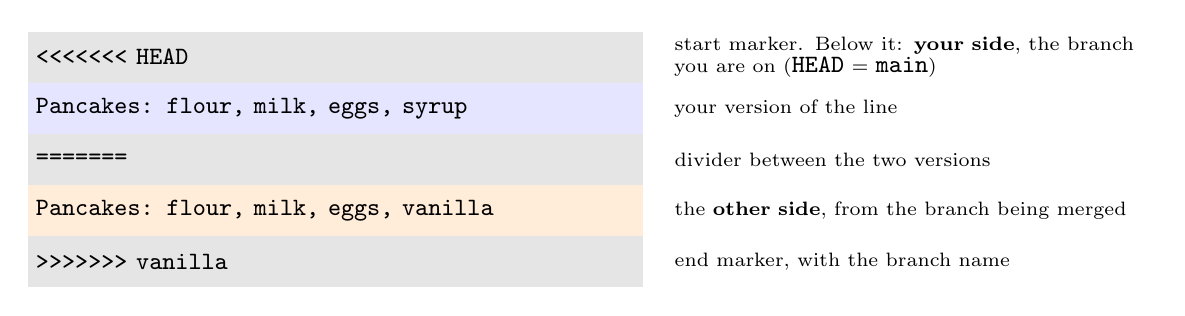
\begin{tikzpicture}[
  ln/.style={font=\small\ttfamily,anchor=west,inner sep=3pt,minimum height=6.5mm,text width=7.6cm},
  note/.style={font=\scriptsize,anchor=west,text width=6.0cm}]
  \node[ln,fill=black!10] (l1) at (0,0)    {<<<<<<< HEAD};
  \node[ln,fill=blue!10]  (l2) at (0,-0.65) {Pancakes: flour, milk, eggs, syrup};
  \node[ln,fill=black!10] (l3) at (0,-1.3)  {=======};
  \node[ln,fill=orange!15] (l4) at (0,-1.95) {Pancakes: flour, milk, eggs, vanilla};
  \node[ln,fill=black!10] (l5) at (0,-2.6)  {>>>>>>> vanilla};
  \node[note] at (8.1,0)     {start marker. Below it: \textbf{your side}, the branch you are on (\code{HEAD} = \code{main})};
  \node[note] at (8.1,-0.65) {your version of the line};
  \node[note] at (8.1,-1.3)  {divider between the two versions};
  \node[note] at (8.1,-1.95) {the \textbf{other side}, from the branch being merged};
  \node[note] at (8.1,-2.6)  {end marker, with the branch name};
\end{tikzpicture}
\caption{Anatomy of a conflict in \code{recipes.txt}. The three marker lines are not part of your text; they must all be removed.}
\label{fig:markers}
\end{figure}

\subsection{Step 3: practise the escape hatch}

Before changing anything, try the safety net. \code{git merge --abort} cancels the whole merge, and Git puts everything back as it was before you typed \code{git merge} (provided the working directory was clean then, as we required):

\begin{lstlisting}
$ git merge --abort
$ git status
On branch main
nothing to commit, working tree clean
$ git merge vanilla                  # the same conflict appears again
\end{lstlisting}

This is the safest way to practise: start a merge, look at the conflict, abort, and try again. \code{--abort} works only while the merge is unfinished; after the final \code{git commit} the merge is done.

\subsection{Step 4: decide and edit}

Open \code{recipes.txt} in your editor. You have three choices: keep your side, keep the other side, or (the usual choice) combine them by writing the line you actually want. Delete the marker lines and leave only the final text. We want both ingredients:

\begin{lstlisting}
Pancakes: flour, milk, eggs, syrup, vanilla
\end{lstlisting}

\begin{pitfall}
The file must contain \emph{no} \code{<<<<<<<}, \code{=======} or \code{>>>>>>>} lines when you are finished. Git will not stop you from committing them, and the file will then be broken. Search for \code{<<<<} before you continue.
\end{pitfall}

\subsection{Step 5: tell Git it is resolved, and finish}

\begin{lstlisting}
$ git add recipes.txt
$ git status
On branch main
All conflicts fixed but you are still merging.
  (use "git commit" to conclude merge)

Changes to be committed:
	modified:   recipes.txt

$ git commit --no-edit
[main 6e9ef86] Merge branch 'vanilla'
\end{lstlisting}

\code{git add} here means ``this file is resolved''. \code{git commit} completes the merge with the prepared message \code{Merge branch 'vanilla'} (drop \code{--no-edit} to edit it; if an editor opens, save and close it). Your ID will differ from \code{6e9ef86}.

\begin{figure}[H]
\centering
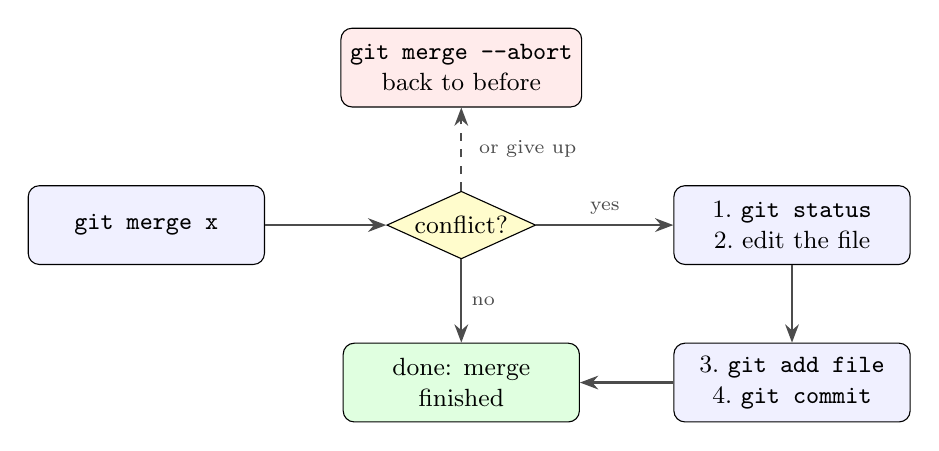
\begin{tikzpicture}[
  blk/.style={draw,rounded corners,fill=blue!6,minimum width=3.0cm,minimum height=10mm,align=center,font=\small},
  dec/.style={draw,diamond,aspect=2.2,fill=yellow!20,align=center,font=\small,inner sep=1pt},
  bad/.style={draw,rounded corners,fill=red!8,minimum width=3.0cm,minimum height=10mm,align=center,font=\small}]
  \node[blk] (m) at (0,0) {\code{git merge x}};
  \node[dec] (c) at (4.0,0) {conflict?};
  \node[blk,fill=green!12] (ok) at (4.0,-2.0) {done: merge\\finished};
  \node[blk] (e) at (8.2,0) {1.~\code{git status}\\2.~edit the file};
  \node[blk] (a) at (8.2,-2.0) {3.~\code{git add file}\\4.~\code{git commit}};
  \node[bad] (ab) at (4.0,2.0) {\code{git merge --abort}\\back to before};
  \draw[link] (m)--(c);
  \draw[link] (c)--node[right,font=\scriptsize] {no} (ok);
  \draw[link] (c)--node[above,font=\scriptsize] {yes} (e);
  \draw[link] (e)--(a);
  \draw[link] (a)--(ok);
  \draw[link,dashed] (c)--node[right,font=\scriptsize] {\ or give up} (ab);
\end{tikzpicture}
\caption{The conflict workflow. You can leave through the red box at any time before the final \code{git commit}.}
\label{fig:flow}
\end{figure}

\begin{quickfact}
Git conflicts not only when two people change the \emph{same} line, but also when changes touch \emph{directly adjacent} lines. If \code{main} had added a new line directly under the \code{Pancakes} line, then merging \code{syrup} (which edits that line) would have conflicted too. Conflicts are normal in teamwork, and they are easy once you have resolved a few.
\end{quickfact}

\begin{quickfact}
\textbf{The other direction.} You can also merge \code{main} \emph{into} a feature branch, to bring it up to date: \code{git switch feature}, then \code{git merge main}. The feature branch is the receiver and \code{main} is unchanged. If you merge in the wrong direction by mistake, do not panic: a finished merge can be undone with \code{git revert -m 1 <merge-commit>} (Lecture 10 shows more ways).
\end{quickfact}

\section{Cleaning up}

A merged branch has done its job. Its commits are now part of \code{main}, so the label can go. In Lecture 4 the command \code{git branch -d} refused to delete an unmerged branch; now it agrees:

\begin{lstlisting}
$ git branch -d crepes shopping syrup vanilla
Deleted branch crepes (was df478ec).
Deleted branch shopping (was 633affa).
Deleted branch syrup (was 0725dd2).
Deleted branch vanilla (was fbed2d3).
$ git branch
* main
\end{lstlisting}

Deleting only removes the label; the commits stay in \code{main}'s history. The usual life cycle of a branch is therefore: \emph{create, commit, merge, delete}.

Run \code{git log --oneline --graph} now: the graph tells the whole story, with three merge commits, each with two parents.

\begin{pitfall}
\textbf{Two common merge mistakes.} (1) Merging in the wrong direction: always \code{git switch} to the receiving branch first, and read the first line of \code{git status}. (2) Starting a merge with uncommitted changes: commit or discard them first, otherwise Git may refuse or mix them into the merge.
\end{pitfall}

\begin{quickfact}
Merging a branch that is already included gives \code{Already up to date.} and changes nothing. (For regretting a finished merge, see the note on \code{git revert -m 1} above.)
\end{quickfact}

\Needspace{10\baselineskip}
\section{Homework 5}

\begin{homework}{5: Merge them all}
From the course folder run:
\begin{lstlisting}
$ bash codeHints/L05/setup_hw5.sh
$ cd practice/hw5
\end{lstlisting}
You get \code{main} (two commits) and four branches: \code{drinks}, \code{desserts}, \code{spicy} and \code{vegan}. Look first with \code{git log --oneline --graph --all --decorate}. Do the tasks \emph{in this order}: the branch you merge first stands above the \code{=======} divider in a later conflict, and the questions in 5.6 depend on that. To start over, run \code{setup\_hw5.sh --reset} from the course folder.

\begin{description}[leftmargin=1.2em,style=nextline]
\item[5.1 First merge] Merge \code{drinks} into \code{main}. (Which kind of merge will it be? Check that Git printed \code{Fast-forward}.)
\item[5.2 Second merge] Merge \code{desserts}. Use \code{--no-edit}.
\item[5.3 Third merge] Merge \code{spicy}. Use \code{--no-edit}.
\item[5.4 The conflict] Merge \code{vegan}. Git reports a conflict in \code{menu.txt}. First look: run \code{git status}, open the file, then cancel with \code{git merge --abort} and check that \code{git status} is clean. Now merge \code{vegan} again and resolve it for real: line 1 of \code{menu.txt} must mention \emph{both} \code{spicy} and \code{vegan} (for example \code{Pizza (spicy, vegan)}), line 2 stays \code{Pasta}, and no marker lines may remain. Add the file and finish with \code{git commit --no-edit}.
\item[5.5 Clean up] Delete the four merged branches with \code{git branch -d}. Only \code{main} should remain.
\item[5.6 Questions] In the file \code{practice/hw5\_answers.txt} (next to the \code{hw5} folder, outside the repository; create it with \code{printf} or \code{echo} in Git Bash, not with a PowerShell redirect) write two lines:
\begin{lstlisting}
above=<spicy or vegan>
merge-commits=<number>
\end{lstlisting}
\code{above} is the branch whose version of the line was \emph{between} \code{<<<<<<< HEAD} and \code{=======} during the conflict in 5.4. \code{merge-commits} is the number of merge commits in \code{main} (look at \code{git log --merges --oneline}).
\end{description}

\textbf{Check yourself:} from the course folder run \code{bash codeHints/L05/check\_hw5.sh}. All \code{PASS}, then compare with the solutions at the end of this lecture (or in \code{solutions/L05/}).
\end{homework}

\section{Summary}

\begin{itemize}
  \item \code{git merge X} brings branch \code{X} into the branch you are on. Switch to the receiver first; start from a clean working directory.
  \item \textbf{Fast-forward}: the receiver has nothing new, so its label just slides forward. \textbf{Merge commit}: both sides have new commits; Git combines them in a commit with two parents.
  \item A \textbf{conflict} means both sides changed the same spot. Open the file, choose or combine the versions, remove the markers, \code{git add}, then \code{git commit}. Use \code{git merge --abort} to cancel.
  \item Afterwards, delete the branch with \code{git branch -d}.
\end{itemize}

\solutionspage

\section*{Solutions to Homework 5}

\begin{lstlisting}
$ bash codeHints/L05/setup_hw5.sh
$ cd practice/hw5
$ git merge drinks
Fast-forward
$ git merge --no-edit desserts
$ git merge --no-edit spicy
$ git merge vegan                     # conflict in menu.txt
$ git status                          # look, then cancel:
$ git merge --abort
$ git merge vegan                     # conflict again, now resolve it
$ cat menu.txt
<<<<<<< HEAD
Pizza (spicy)
=======
Pizza (vegan)
>>>>>>> vegan
Pasta
\end{lstlisting}

Edit \code{menu.txt} so that it contains exactly

\begin{lstlisting}
Pizza (spicy, vegan)
Pasta
\end{lstlisting}

then finish and clean up:

\begin{lstlisting}
$ git add menu.txt
$ git commit --no-edit
$ git branch -d drinks desserts spicy vegan
$ git log --merges --oneline          # three lines
$ printf 'above=spicy\nmerge-commits=3\n' > ../hw5_answers.txt
\end{lstlisting}

\textbf{5.1.} \code{main} had no commits of its own beyond the shared start, so Git fast-forwarded: no merge commit, and \code{main} now points where \code{drinks} points. If you used \code{--no-ff}, you get an extra merge commit and the checker reports four merges.

\textbf{5.2 and 5.3.} \code{main} had moved (it contains \code{drinks}), so Git made a merge commit each time. \code{desserts} adds a new file and \code{spicy} edits \code{menu.txt}, which \code{main} has not changed, so there is nothing to resolve.

\textbf{5.4.} \code{spicy} and \code{vegan} both changed line~1 of \code{menu.txt}, which makes a conflict. Between \code{<<<<<<< HEAD} and \code{=======} stands \emph{your side}, the branch you are on. Because \code{spicy} was merged into \code{main} first, that is the spicy version, which is why the answer to 5.6 is \code{above=spicy}. After the abort \code{git status} says \code{working tree clean}: the merge never happened, and you can try again. Any text that mentions both words on line~1 passes the checker. The line \code{Pasta} was not part of the conflict and stays unchanged. Check that no marker line is left with \code{grep -n '<<<<\textbackslash|====\textbackslash|>>>>' menu.txt} (it should print nothing).

\textbf{5.5.} \code{git branch -d} works because every branch is now fully merged. Had Git refused, that would indicate an unmerged branch.

\textbf{5.6.} Three merge commits: \code{desserts}, \code{spicy} and \code{vegan}. The \code{drinks} fast-forward made none.

\Needspace{8\baselineskip}
\textbf{Common mistakes.}
\begin{itemize}
  \item Merging \code{vegan} before \code{spicy}. Then \code{vegan}'s version stands above the divider, but the checker expects \code{above=spicy}, so follow the order of the tasks.
  \item Committing with the marker lines still in the file. Open the file and check.
  \item Running \code{git commit} without \code{git add menu.txt} first: Git refuses and says the path is unmerged.
  \item Running \code{git merge --abort} \emph{after} the final commit: it no longer applies. Use \code{setup\_hw5.sh --reset} and start again.
\end{itemize}


\end{document}
